\documentclass[12pt, a4paper]{article}  


\usepackage{amsmath,amsfonts,amssymb,amsthm,mathtools}  
\usepackage{graphicx}

\usepackage{fontspec}         
\setmainfont{Helvetica} 
\newfontfamily{\cyrillicfonttt}{Helvetica}
\newfontfamily{\cyrillicfont}{Helvetica}
\newfontfamily{\cyrillicfontsf}{Helvetica}   

\usepackage{unicode-math}  
\setmathfont{Asana-Math.otf}   
 

\usepackage{polyglossia}      
\setdefaultlanguage{russian}  
\setotherlanguage{english}    
\usepackage{graphicx}                  % Для вставки рисунков
\usepackage{graphics} 
\graphicspath{{images/}{pictures/}}    % можно указать папки с картинками
\usepackage{wrapfig}                   % Обтекание рисунков и таблиц текстом
\usepackage{subfigure}                 % для создания нескольких рисунков внутри одного
\usepackage{tabularx}            % новые типы колонок
\usepackage{tabulary}            % и ещё новые типы колонок
\usepackage{array}               % Дополнительная работа с таблицами
\usepackage{longtable}           % Длинные таблицы
\usepackage{multirow}            % Слияние строк в таблице
\usepackage{float}               % возможность позиционировать объекты в нужном месте 
\usepackage{booktabs}            % таблицы как в книгах!  
\renewcommand{\arraystretch}{1.3} % больше расстояние между строками


\begin{document}


\begin{figure}

\begin{minipage}[h!]{0.3\textwidth}

\includegraphics[width=\textwidth]{pop3.pdf}
\end{minipage}
\begin{minipage}[h!]{0.3\textwidth}
\includegraphics[width=\textwidth]{pop5.pdf}
\end{minipage}
\begin{minipage}[h!]{0.3\textwidth}
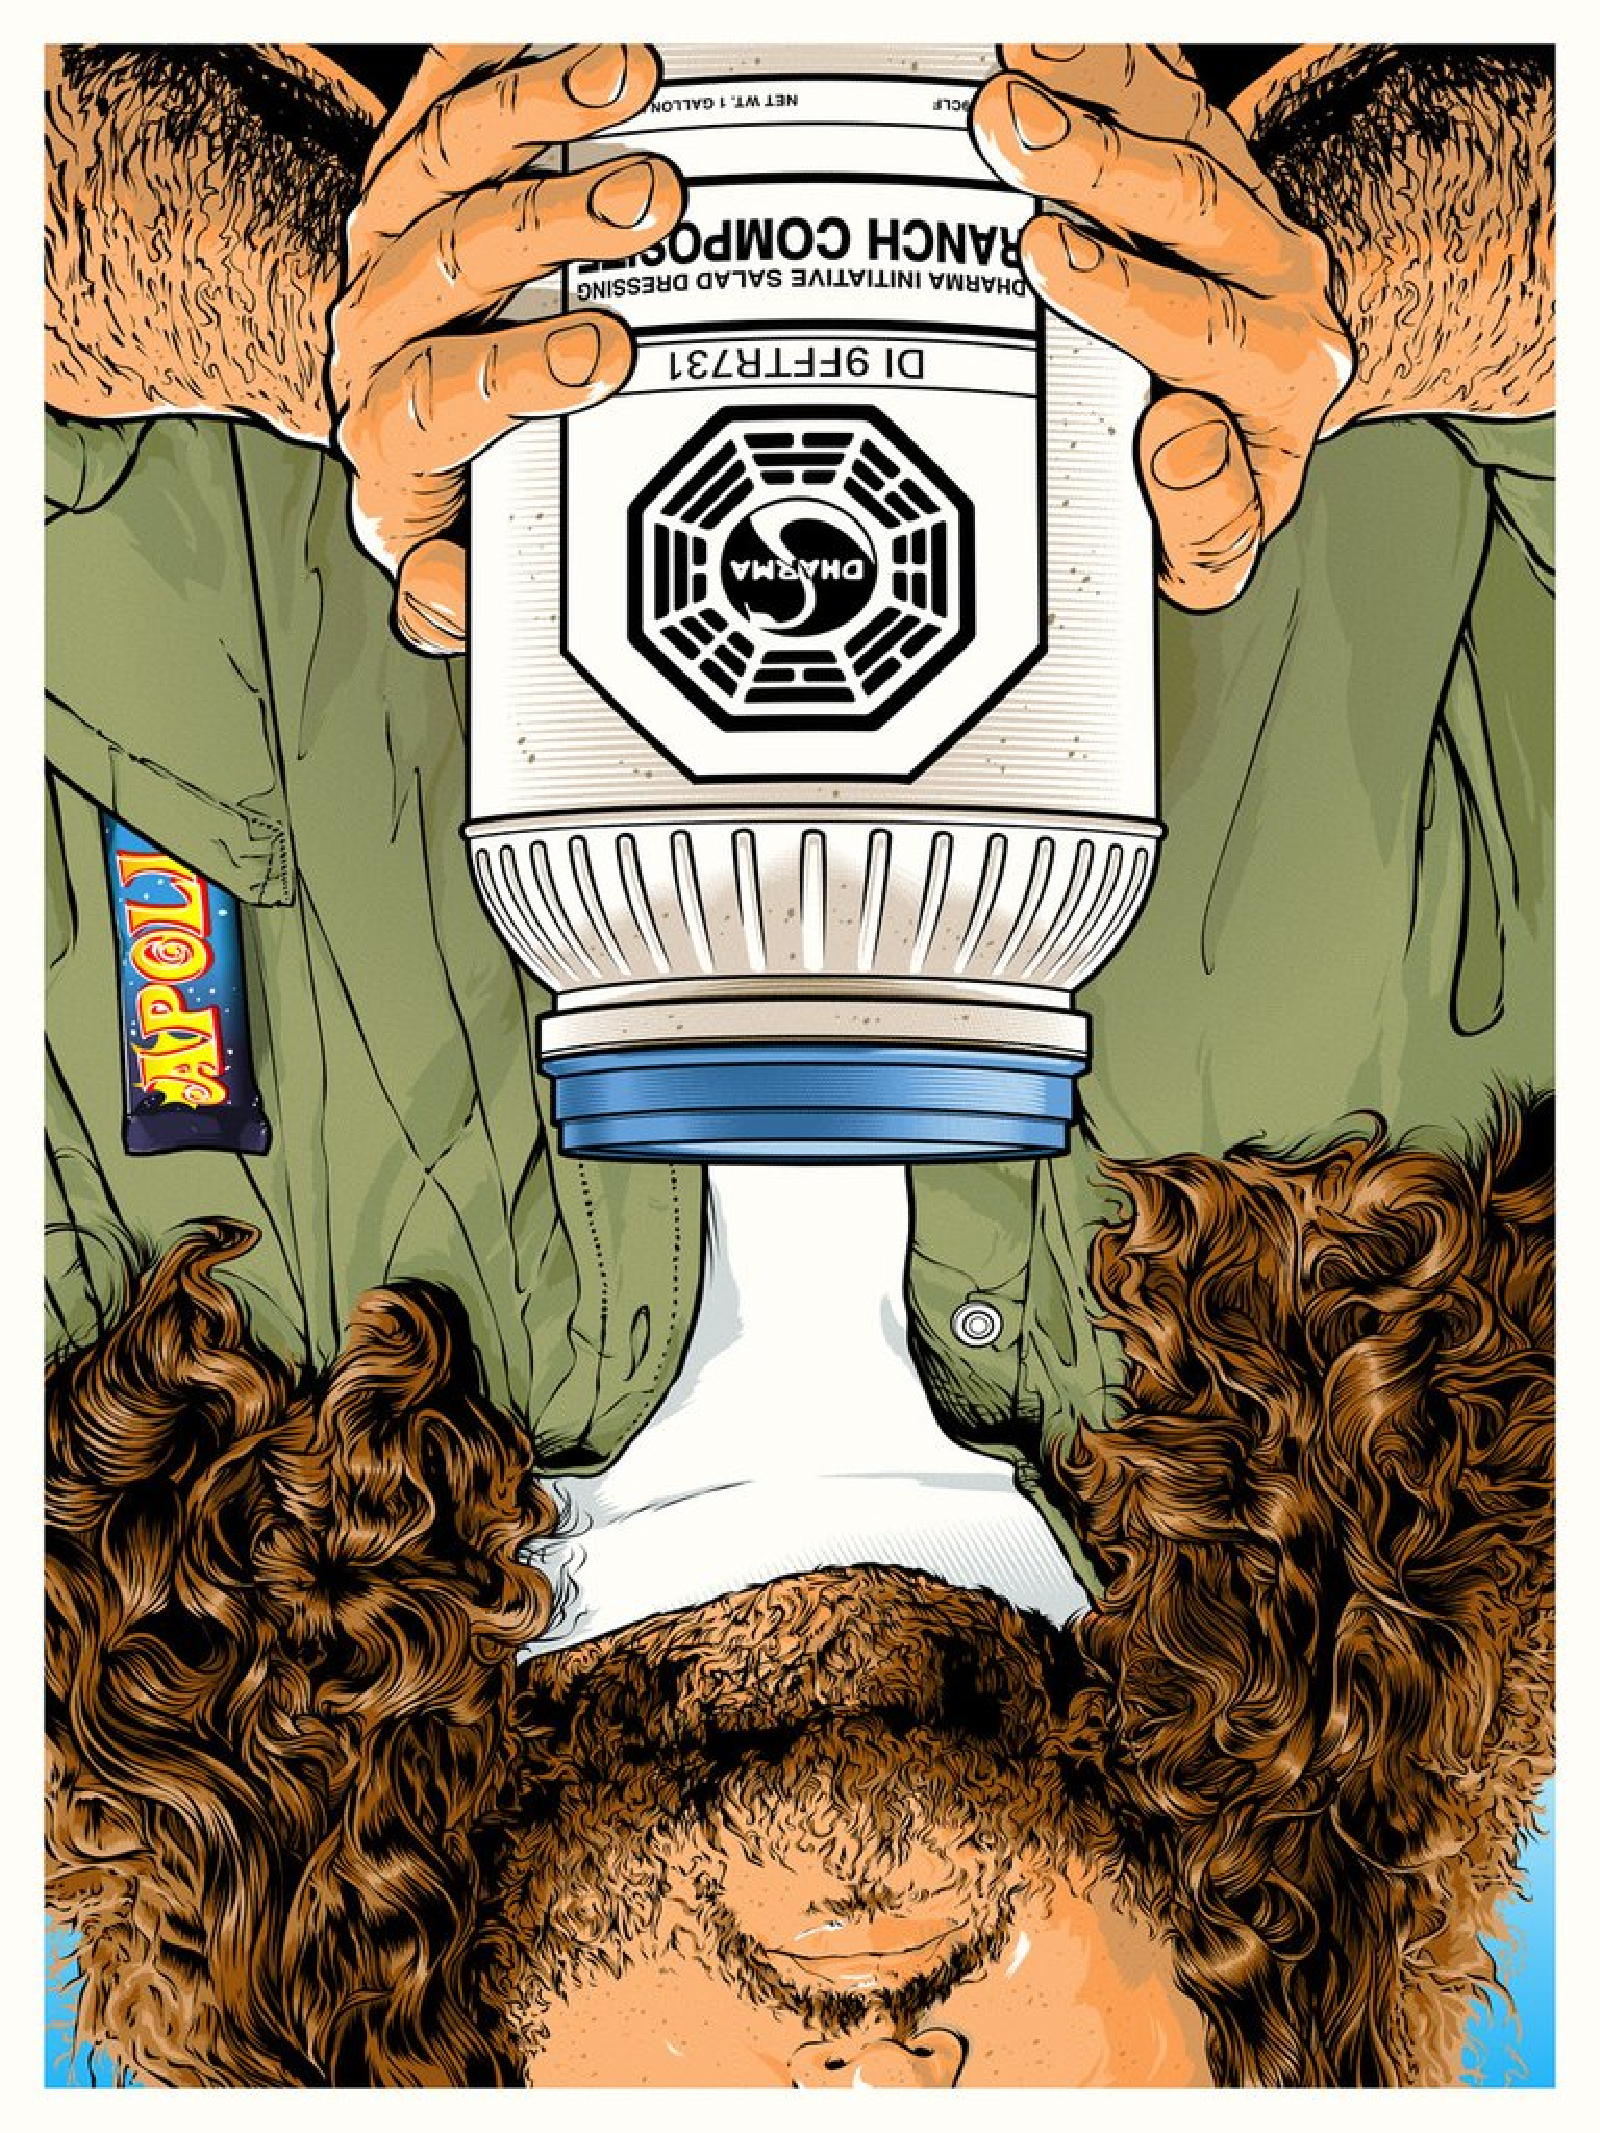
\includegraphics[width=\textwidth, angle=180]{pop10.pdf}
\end{minipage}
\vfill

\begin{minipage}[h!]{0.3\textwidth}
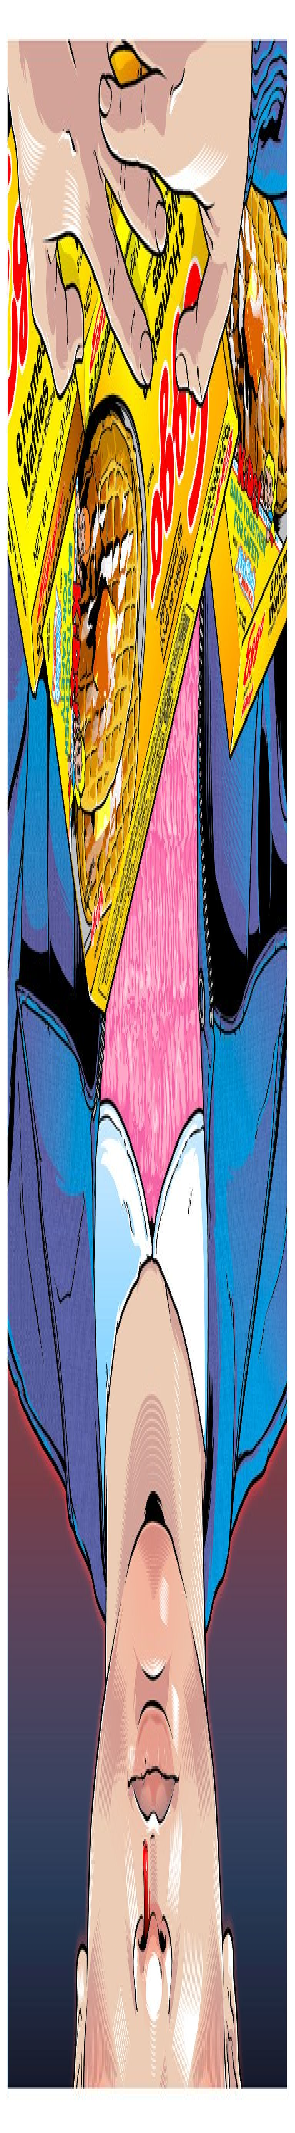
\includegraphics[height=5.49cm,width=4.2cm,angle=180]{pop2.pdf}
\end{minipage}
\begin{minipage}[h!]{0.3\textwidth}
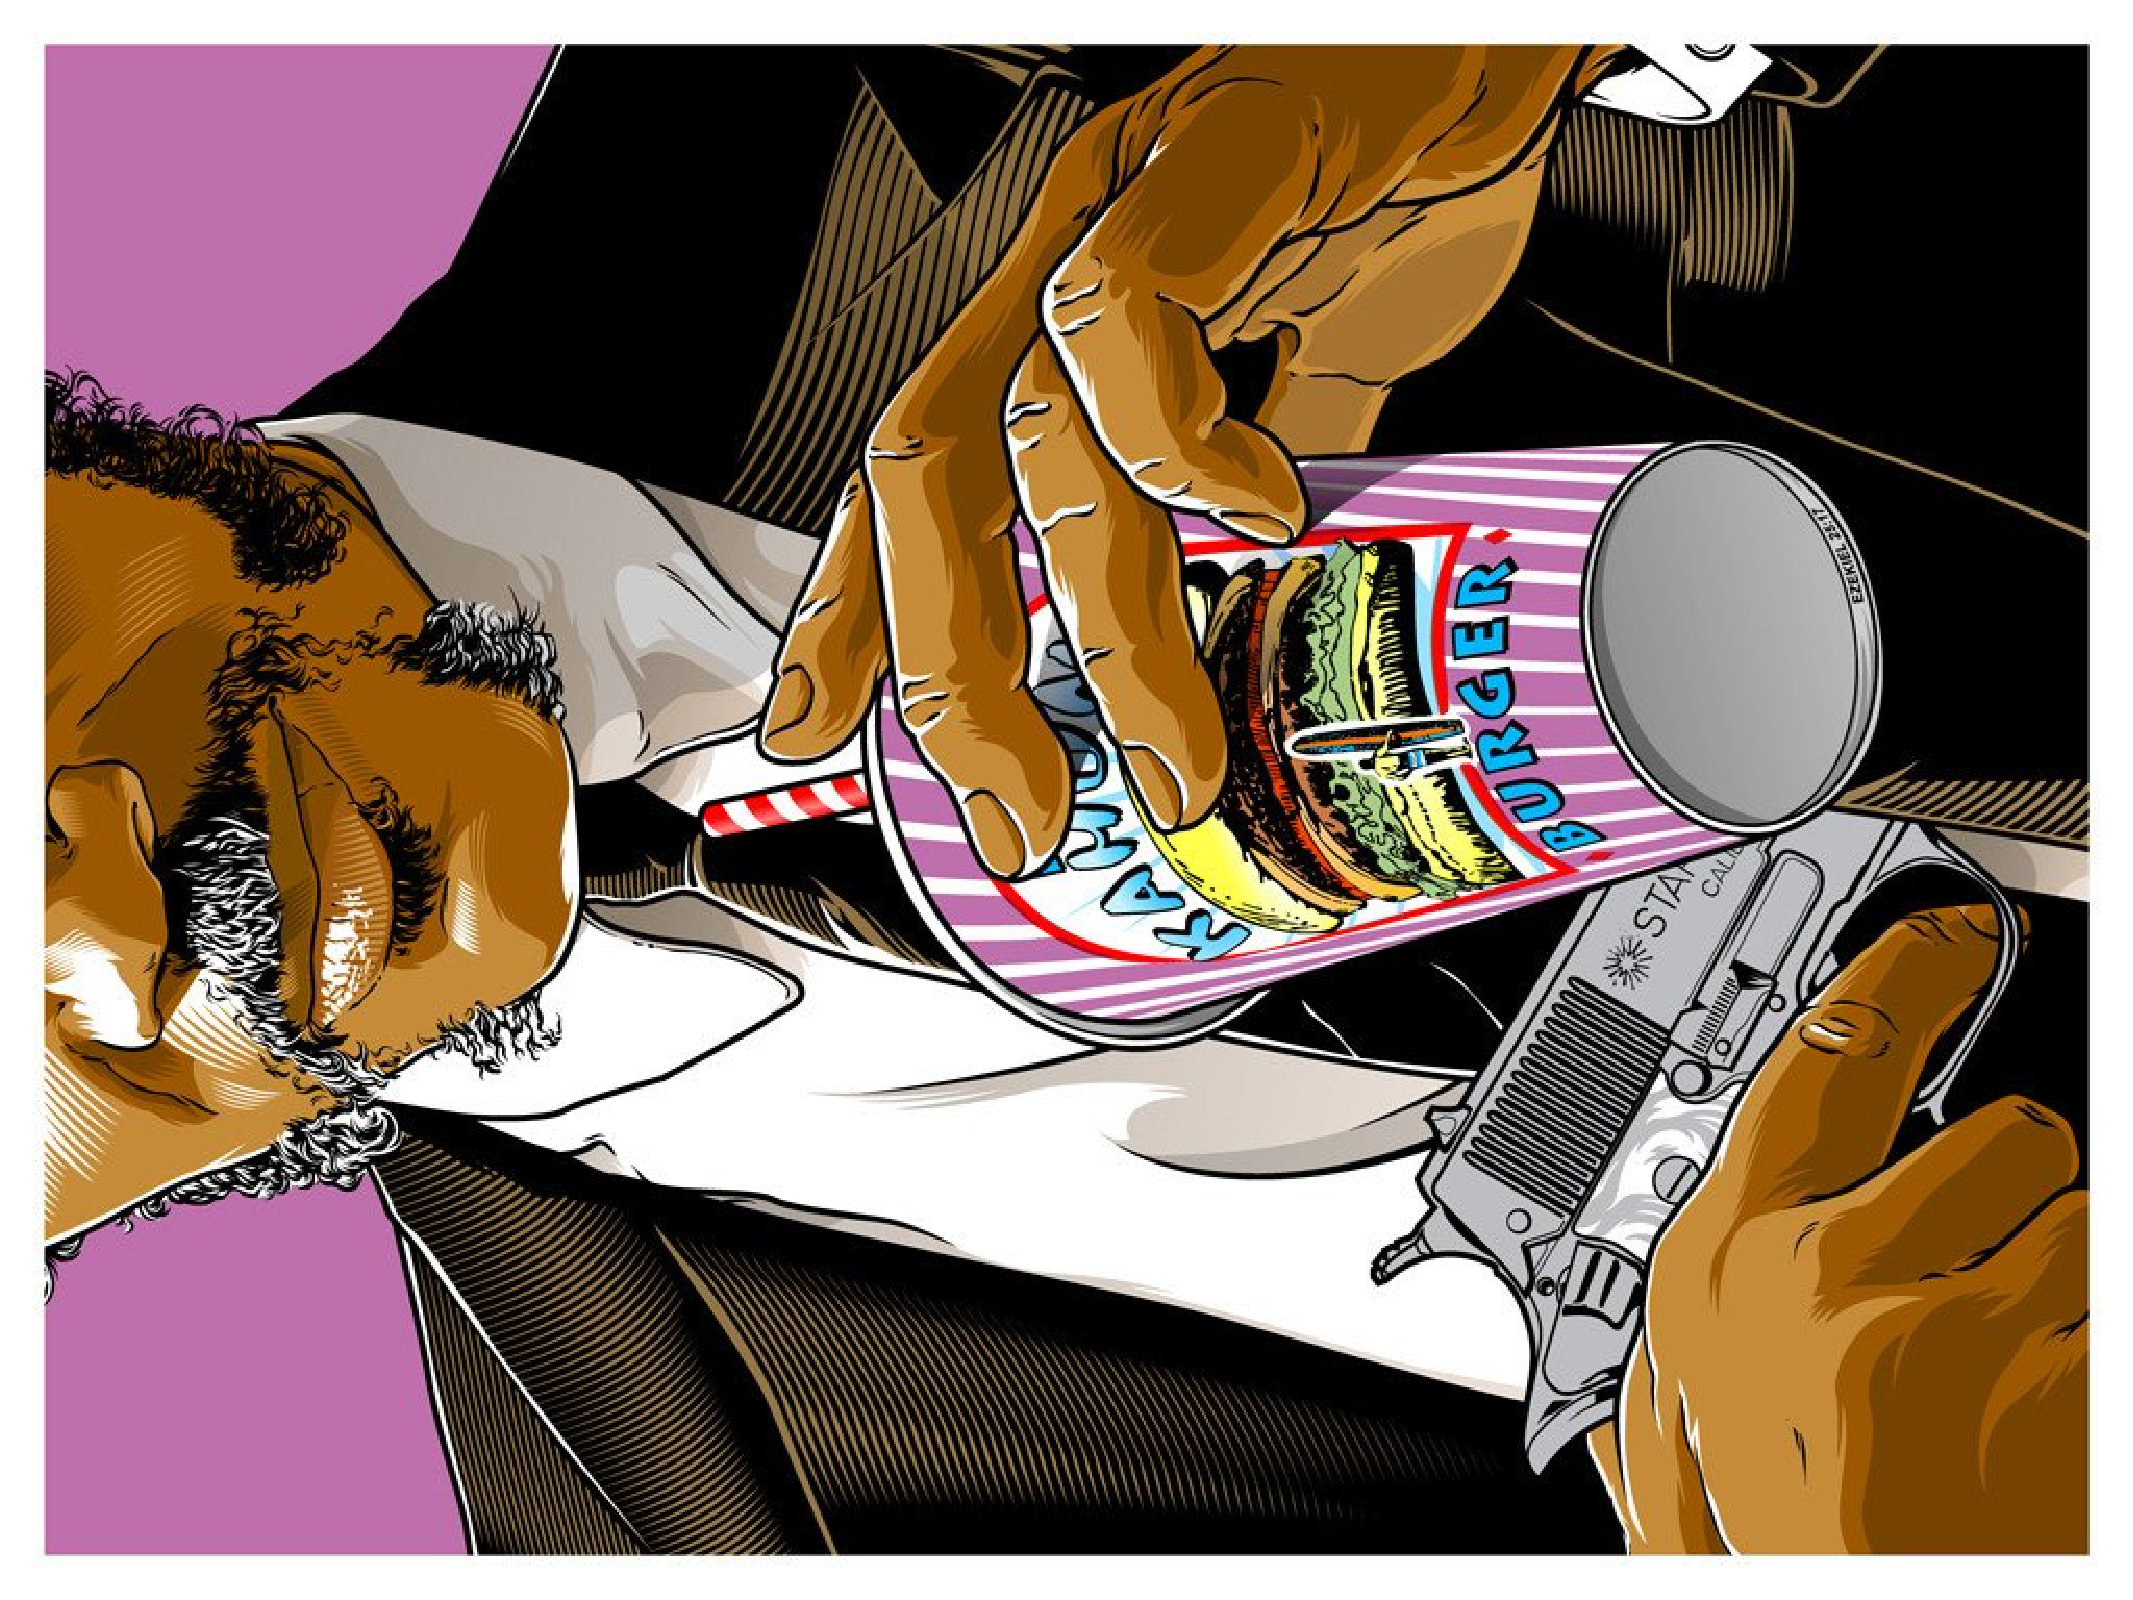
\includegraphics[height=4.1cm,width=6cm,angle=270,keepaspectratio]{pop1.pdf}
\end{minipage}
\begin{minipage}[h!]{0.3\textwidth}
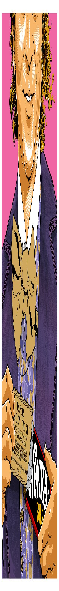
\includegraphics[height=5.5cm,width=4.1cm]{pop7.pdf}
\end{minipage}
\caption{Это что, поп-арт?}
\end{figure}

\end{document}
